\documentclass[twoside,11pt]{article}

\usepackage{../Style/feuille-tp}
\usepackage{lscape}

\formation{IUT - Département Informatique}
\matiere{Théorie des langages -- 2013-2014}
\titre{Langages algébriques}
\sigle{MATHS \\ S4 - TDL}

\basdepage{S4 - Maths- Théorie des langages}


\sloppy

\begin{document}
\maketitle

\section{BNF}

Backus-Naur Form, inventée pour les besoins du groupe de travail ALGOL (1960).

\subsection{La BNF ... en BNF}

\begin{lstlisting}[frame=single, numbers=left]
syntax     ::=  { rule }
rule       ::=  identifier  "::="  expression
expression ::=  term { "|" term }
term       ::=  factor { factor }
factor     ::=  identifier |
                quoted_symbol |
                "("  expression  ")" |
                "["  expression  "]" |
                "{"  expression  "}"
identifier ::=  letter { letter | digit }
quoted_symbol ::= """ { any_character } """
\end{lstlisting}

\subsection{Exercices}

\paragraph{Le langage PL/0} de N. Wirth est décrit par une grammaire
de type E-BNF (extended BNF). Ecrivez quelques programmes dans ce langage.
{\small
\begin{lstlisting}[frame=single,numbers=left]
 program = block "." .
 
 block =
     ["const" ident "=" number {"," ident "=" number} ";"]
     ["var" ident {"," ident} ";"]
     {"procedure" ident ";" block ";"} statement .
 
 statement =
     ident ":=" expression
     | "call" ident
     | "begin" statement ";" {statement ";"} "end"
     | "if" condition "then" statement
     | "while" condition "do" statement .
 
 condition =
     "odd" expression
     | expression ("="|"#"|"<"|"<="|">"|">=") expression .
 
 expression = ["+"|"-"] term {("+"|"-") term} .
 
 term = factor {("*"|"/") factor} .

 factor =
     ident
     | number
     | "(" expression ")" .

\end{lstlisting}

\paragraph{Exercice.} Voici des exemples de déclarations de type en 
langage Pascal. Fournissez une grammaire qui couvre au moins
les exemples :

\begin{verbatim}
type chaine = array [1 .. 30] of char;
type date = record 
               jour : 1..31;
               mois : 1..12;
               annee : integer
            end;
type personne = record
                  nom, prenom : chaine;
                  naissance   : date
                end;
\end{verbatim}

                   
\paragraph{Exercice. } Voici un programme écrit dans un langage jouet
\begin{verbatim}
function fac(n)
  local r = 1, i
  for i = 1 to n do
    let r = r * i
  endfor
  return r
endfunction

let encore = 1
while encore == 1 do
  print "valeur de n ? "
  read n
  if n < 0 
  then 
     print "n est négatif"
     let encore = 0
  else 
     let r = fac(n)
     print "factorielle ", n, " = ", r
  endif
endwhile  
\end{verbatim}

Fournir une description du langage en BNF étendue.

\newpage
\section{Diagrammes syntaxiques}
Exemple : les expressions arithmétiques.

{\scriptsize

\url{http://commons.wikimedia.org/wiki/File:Diagrammes_Syntaxiques.png}
}

\begin{center}
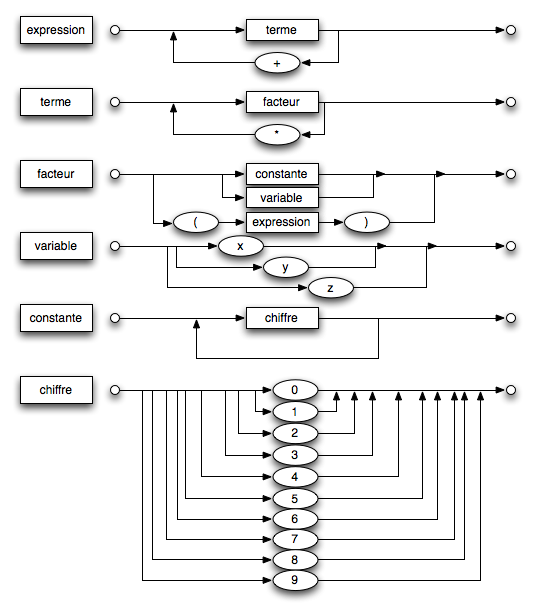
\includegraphics[width=\linewidth]{../images/Diagrammes_Syntaxiques}
\end{center}

\paragraph*{Exercice. } Convertir la description de PL/0 en diagrammes syntaxiques.

\newpage
\section{Descente récursive, un exemple}

Le programme ci-dessous analyse une expression arithmétique, et en
fournit une paraphrase.

% \begin{landscape}

\lstinputlisting[language=c++,frame=single,numbers=left,breaklines=true]{../src/lecture-expr.cxx}

% \end{landscape}

Résultat : 

\lstinputlisting[frame=single,breaklines=true]{../src/lecture-expr.run}

\end{document}
